
\chapter{Introduction}
\label{chapter1}

% 1.1.
\section{Plasma Science}

This thesis is multidisciplenary by nature, incorporating aspects of mathematics, physics and computer science throughout 
the various challenges faced in reaching the conclusions we have. 


Before burying ourselves in the thick of our results we 
will cover the requisite knowledge for working in the plasma science simulation space. First we will discuss what 
the physical object of our attention (``plasma'') actually is, with a brief discussion on the design of fusion reactors, where we will 
emphasise the structures that specifically relate to our interests. In the background chapter we will expound on this by 
building the mathematical theory underpinning physical processes within the fusion reactor, providing us a way to reason
about the behaviour of plasma (and related processes) inside a fusion reactor, or, more accurately, approximate their behaviour 
via simulation.




% 1.1.1.
\subsection{I'm a Mathematician... what is ``plasma''?}

While an initially daunting topic, fear not fearful mathematician, for many of the inherently physical 
behaviours in plasma science we require can be expressed in terms of our dearest mathematical expressions -- differential equations! 
But first, what actually is ``plasma''? Webster's dictionary defines plasma to be ``a green faintly translucent quartz'' \cite{websters_plasma}. 
While I'm sure there isn't no relation between crystals and our investigations, this is unfortunately, not the recipient of our affection. 

When plasma is referred to in everyday conversation it is often noted as being the ``4th state of matter''. To introduce slightly more rigour,
plasma is an extension of the gaseous state of matter, where its energy (read: temperature) is increased sufficiently high that the electrons 
are no longer bound by the electromagnetic force to the atom's nucleus \cite{basics-of-plasma-astrophysics}. The resulting substance is a ``pool'' of cations (the positively charged nuclei), and 
electrons (negatively charged), that exhibits interesting properties. It is these properties that we seek to exploit in the search for controlled, 
sustainable fusion reactions.

Plasma is abundant in nature -- just not in many places that we as Humans commonly look. Stars are the most immediate example of matter in a plasma state, 
and are readily viewable (at least for half the day). Lightning strikes are paths through the atmosphere which are ionised, 
and neon signs work by heating Neon gas within a tube to ionise it \cite{plasma-lightning}.

The question then is, what is ``fusion'', and how does this relate to plasma? The answer comes back to energy. Analogously to a fission reaction, 
where energy is released through the division of atoms, one can also fuse two separate atoms together and have large amounts of energy emitted 
as a bi-product of that fusion. It is (essentially) this extra energy that we wish to harness when harvesting energy from a fusion reactor.

While there are no shortages of elements that can theoretically be used to fuel a fusion reactor, the one most commonly associated with fusion is Deuterium -- a stable isotope of Hydrogen that 
has a neutron in its nucleus (whereas a 'standard' Hydrogen atom contains only a single proton). Analogously, Tritium is an isotope of Hydrogen
that has two neutrons in its nucleus (though is much less stable). Consider the fusion of a Deuterium atom with a Tritium atom:
\[ \prescript{2}{}{\text{H}} + \prescript{3}{}{\text{H}} \stackrel{\text{(fusion)}}{\to} \prescript{4}{}{\text{He}} + n + 17.59 \, \text{MeV} \]

Here two Hydrogen isotopes fuse together to form a single Helium-$4$ atom, and in the process of doing so release 
a single neutron and $17.59$ MeV of energy. This excess energy is what is so attractive about fusion processes as a sustainable 
energy source -- for such little input we receive a substantial amount of energy, and at that, using one of the most abundant 
resources available on Earth; water.

The question then becomes, how do we drive this fusion process? If two atoms can fuse as such, why do we not 
see atoms fusing everywhere around us accompanied by violent explosions destroying all that we've 
come to know and love? The answer is that we kind of do. In fact, we see this happening everyday --
for those of us fortunate enough to be able to see the sun that is. Our sun 
is a large ball of plasma where an estimated $9.3 \times 10^{37}$ fusion reactions are expected to occur every second \cite{nasa-sun-fusion}, 
and is one of the easiest examples of both plasma as a state of matter, and of a self-sustaining fusion reaction.

How then do two hydrogen atoms fuse? The nucleus of an atom (consisting of positively charged 
protons, and neutral neutrons) is positively charged, and so two atoms' nuclei will repel each other due to the Coulomb force when pushed together. This is the force 
we have to overcome to enable a fusion reaction to take place (and what stops the world around us burning!). To overcome this the process is relatively ``simple'' -- 
we just increase the energy of our atoms so that when they collide they collide with enough energy to overcome this force, allowing the strong force to become
dominant, fusing the two atoms. When we energise a mass (take a gas here) of atoms enough, they become ionised however, which is 
exactly the state of plasma we described earlier. In other words, if we want to reason about the creation, sustainment, and effects of 
fusion reactions, we need first to understand the dynamics of plasma, the medium in which the fusion reactions take place. From this comes a plethora of questions, ranging from 
``how do we generate such a plasma?'' to ``how do we reliably control such a plasma'' and ``how do we harvest energy from a plasma''? Alas, we 
digress however, as we do not seek to solve the big problems in fusion science in this here mere mortal thesis. Instead, now equipped 
with at least a passing knowledge of what constitutes a ``plasma'' state and what it means for a fusion reaction to take place, 
we will humbly delve into the inner workings of fusion reactor terminology and design.


% 1.1.2.
\subsection{Fusion Reactor Design 101}

Here we will discuss the important structural aspects of a tokamak fusion reactor. The term ``tokamak'' is a 
Russian acronym which translates as ``toroidal chamber with magnetic coils'' \cite{iter-tokamak-acronym}. Aptly, a tokamak is a toroidal 
object which is used as a vessel for plasma which is driven via external magnetic coils. There are two main angular components 
to a tokamak - components working in the ``toroidal'' (around the major radius, $R$, of the tokamak), and those working in the 
``poloidal'' direction (around the minor radius, $a$, of a cross section of the tokamak). Thus, we will often reason about 
various physical concepts (such as magnetic fields, current densities) in terms of one of these. Though, in fact, we will 
often ignore the toroidal component - these are often abstracted away under the guise of an axisymmetry assumption, which assumes 
that any changes in the plasma with respect to the toroidal angle are diminishing, i.e., $\pdv{\phi} = 0$. We let $\theta$ denote poloidal angles, 
and $\phi$ the toroidal angles. When we refer to $(x,z)$, we will be referring to offsets within a poloidal cross section. 
Refer to figure \ref{dimensions} for a graphic distinguishing toroidal from poloidal components.

\begin{figure}[h!]
    \centering
    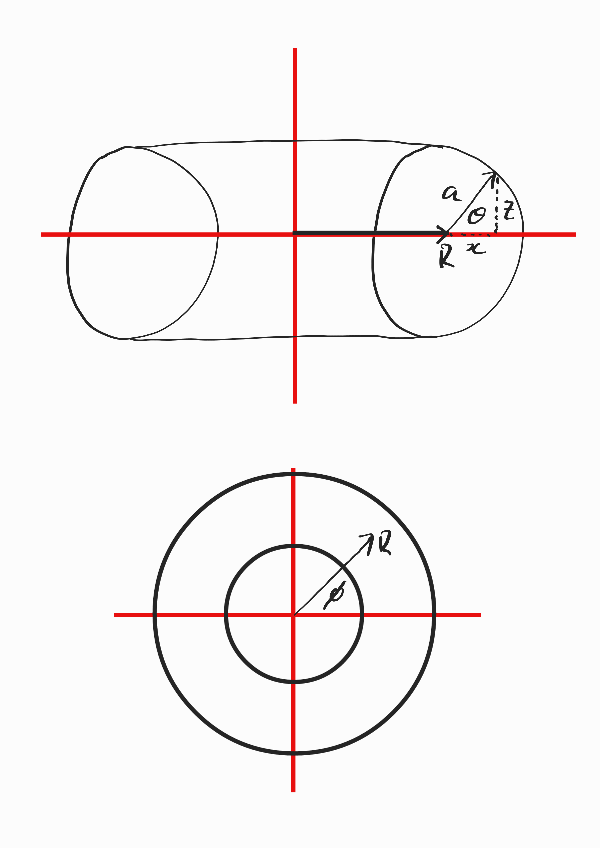
\includegraphics[scale=0.5]{imgs/c1/dimensions.png}
    \caption{The top half depicts poloidal cross section factors, whereas the bottom shows toroidal components. }
    \label{dimensions}
\end{figure}

We draw specific attention to the difference between poloidal and toroidal magnetic flux. In this thesis we will concern 
ourselves primarily with poloidal magnetic flux, which is what controls lateral ``movement'' of plasma within the tokamak - 
which is central to the problem of confinement (pun intended). See figure \ref{flux-functions} for a comparison.

\begin{figure}
    \centering
    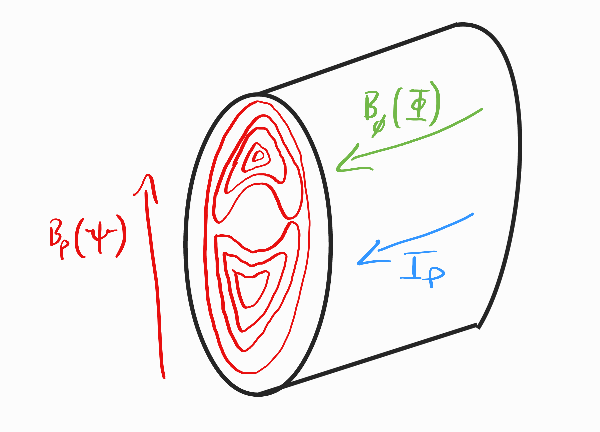
\includegraphics[scale=2.0]{imgs/c1/flux-functions.png}
    \caption{Emphasising the difference between the poloidal and magnetic fields. The flux function symbols associated with each are 
    also provided. Alongside this we show the plasma current flow for good measure.}
    \label{flux-functions}
\end{figure}

We control fusion reactors via a series of (meticulously!) placed solenoids around the external of the reactor. These are positioned 
such that certain solenoids can be used to shape either the toroidal or poloidal magnetic field. Current is passed through these,
the strength of which drives the strength of the resultant magnetic field, and the direction of which is determined by the 
``right hand rule'' if you recall high school physics exams with everyone staring at their hands. We see a depiction of these solenoids 
and their effect on the poloidal and toroidal magnetic fields in figure \ref{solenoids}. Note that we have ignored one set of solenoids which accompany these, which are placed 
following the contours of the toroidal direction, and are used for more fine grained control of the poloidal magnetic flux - these are 
largely irrelevant for our purposes however, and are annoying to draw, and so are omitted from the graphic.

\begin{figure}[h!]
    \centering
    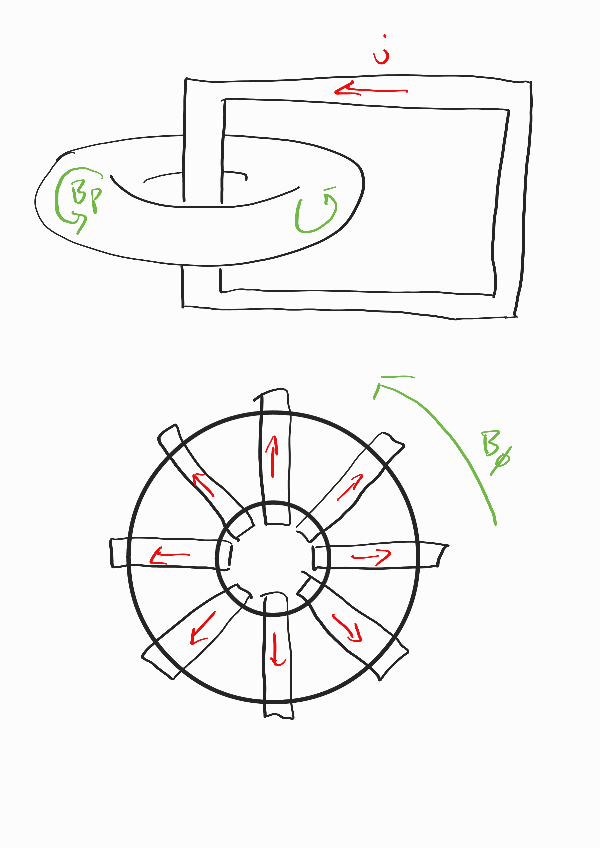
\includegraphics[scale=0.5]{imgs/c1/solenoids.png}
    \caption{Solenoids which control the poloidal and toroidal magnetic fields.}
    \label{solenoids}
\end{figure}\newpage

\subsubsection{Reactor Geometry}
In reality, reactors do not have such nice geometry as the above diagrams (if we take shaky hand-drawn pictures to have ``nice'' geometry). Figure \ref{fig:east-geometry}
shows a 3D model of the EAST reactor, showing the irregularities in the shape of the cross section that appears in a real reactor. These 
engineering decisions made here are interesting and could be (and have been) the subject of their own research! For our purposes however, we will 
assume that our tokamak is either a torus with an elliptic cross section, or even simpler, a cylinder with elliptic cross section. These act 
as approximations to a real tokamak's design to make simulation simpler - it is the ``spherical cow'' model for fusion reactors.

\begin{figure}[h!]
    \centering
    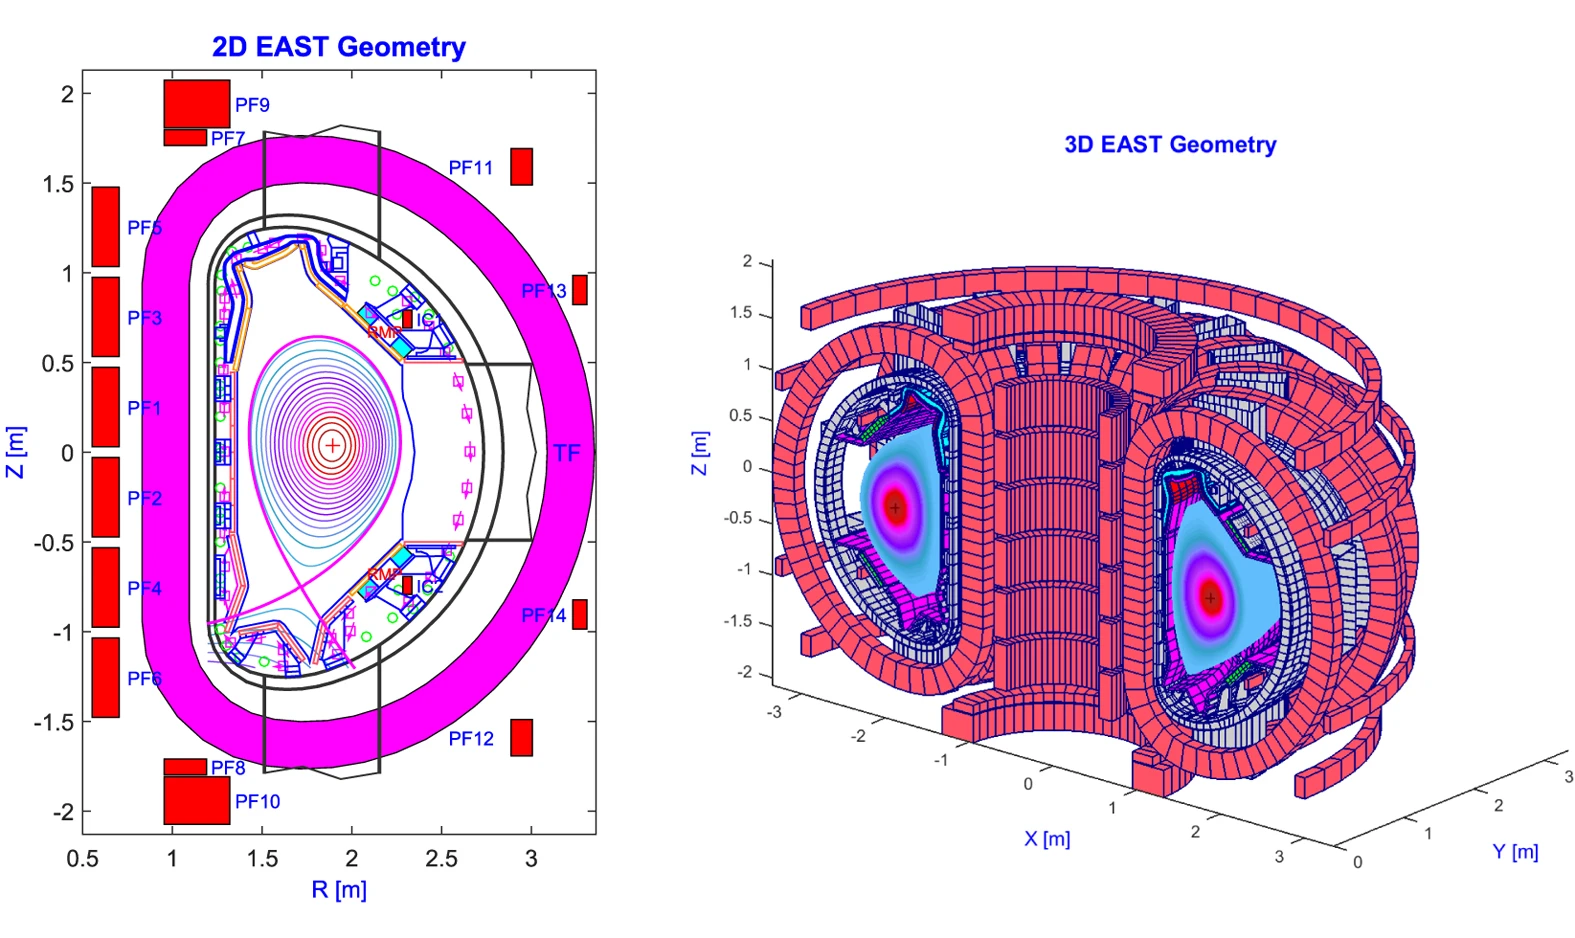
\includegraphics[scale=0.2]{imgs/c1/east-cross-section.png}
    \caption{EAST fusion reactor geometry. This is a 3D model of its cross section, highlighting the irregular shape \cite{east-geometry-article}}
    \label{fig:east-geometry}
\end{figure}

\subsubsection{Runaway Electrons}
We make one last note on runaway electrons. If a tokamak were Alexander Hamilton, then runaway electrons would be Aaron Burr. Or Hamilton. Or time? 
Whatever your interpretation of Lin Manuel-Miranda's musical epic suggests is the enemy. These high energy particles have the 
potential to be highly damaging to a reactor. They have the ability to directly damage equipment within the reactor (such 
as instruments that are plasma-facing), can erode the inside protective layers of the tokamak, can 
disrupt the dynamics of the plasma, and more. In fact it is runaway electron mitigation 
techniques which are at least part of the reasoning for having such an irregularly shaped 
cross section as that adopted by the EAST reactor (and many more ``modern'' reactors). We will talk more about runaway electrons in chapter \ref{chapter2}.

Now that we are experts in fusion reactor design (who needs a physics degree, right?), we can proceed to talk about the 
afflictions that modern day fusion reactors face and what this humble thesis attempts to tackle.

% 1.2
\section{What problem does this thesis address?}

The core problem that this thesis is built around is introduced by Hole and Malaquias \cite{malaquias-matthew}.
In a tokamak, external solenoids along with heating elements within the reactor are 
what drive the primary current within a plasma. In a reactor operating in the DC regime, this is 
characterised by being a constant, unidirectional current. However, when operating in AC mode, 
this naturally becomes oscillatory. At every current reversal there is necessarily a quiescent phase 
for the plasma current, where $I_{p} = 0$. At this point we would anticipate there to be no plasma density,
as a result of there being no current to drive its temperature, however experimental results from ISTTOK (the 
reactor which provides Hole and Malaquias, and us, data - more specific details for it are provided in chapter 
\ref{chapter5}) disagree with this expectation. 
Notably, reactors such as the CT-6B tokamak identify through experiment the presence of coexisting anti-parallel 
currents in the ramp down phase - directly contradicting ISTTOK's observations \cite{huang-ct-tokamak}. 
Summarily, there is no consensus in the community surrounding three central issues:
\begin{itemize}
    \item Why does there exist a residual plasma density when there is seemingly nothing to drive it? (i.e. $I_p = 0$)
    \item Why do we see an increase in runaway electron generation during the ramp down phase ?(and partly during 
    ramp up, though we will note on this missing data in chapter \ref{chapter2})?
    \item There is experimental evidence that both supports and discounts the existence of anti-parallel current
    formation during the ramp down phase. What could drive this, and is there theoretical support for either side?
\end{itemize}

\begin{figure}[h!]
    \centering
    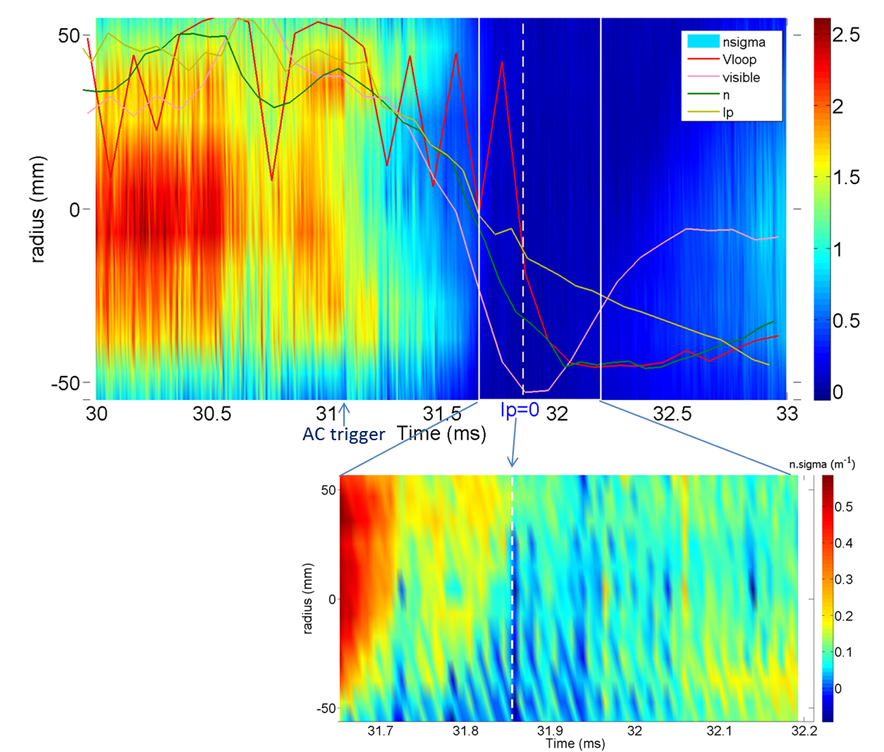
\includegraphics[scale=1]{imgs/c1/residual-plasma.png}
    \caption{ISTTOK data showing the existence of a residual plasma density despite the plasma current $I_p$ and 
    $v_{\text{loop}}$ being negligible \cite{malaquias-matthew}.}
\end{figure}

It is hypothesised by Hole and Malaquias that this residual plasma density is the result of 
persistent runaway electron populations in the plasma. It is further suggested that these populations
are driven by some mechanism reuslting from the ramp down phase - we discuss runaway electron generation 
mechanisms in chapter \ref{chapter2}. As we noted however, experiments are inconsistent on the question of 
the existence of anti-parallel current channels (concurrent positive and negatively oriented current densities) in the plasma. 
In ISTTOK we note that the $V_{\text{loop}}$ of the plasma (essentially the plasma's voltage) is vanishing as the plasma 
current approaches $I_p = 0$. This combined with the observation that the pressure density profile, as measured 
by the ISTTOK heavy ion beam diagnostics team, show non-vanishing pressures within the plasma, indicating 
the presence of a residual plasma even as the plasma current vanishes. This same pressure density profile 
also shows no evidence of the coexistence of anti-parallel currents.

\subsubsection{What results do we seek?}
Our broad scope goal is to simulate the behaviour of a current reversal within a tokamak, with the intent 
of identifying indicators of runaway electron generation, or support for the presence of anti-parallel current formation
- in effect, to provide some insight into the answers behind any of the three points raised above. 
More specifically, however, we will develop theory around simulating the behaviour of a ramp down phase, necessarily a time evolution, when 
the tools we have available to us are characteristically time independent. From this we will develop a model 
which targets specifically the scenario that we have access to current density profile data, and from this 
derive information about the pressure density profile and the poloidal magnetic flux. We will run simulations 
for a contrived tokamak to observe some theoretical results, before applying what we've learned to data 
made available by the ISTTOK project. From this we will attempt to draw inference about the behaviours listed 
above, and note any limitations that may exist on our model.

% 1.3.
\section{Project Progression}

This project being inspired by work done by Hole and Malaquias and the scope for the project defined explicitly, 
we first begun with a review of existing theoretical work done in simulating current reversals in tokamaks. These 
efforts led to the discovery of Wang's paper \cite{wang-analytic-solution}, which provided an analytic solution 
to a variation of the Grad-Shafranov equation constructed specifically for the modelling of equilibrium in 
current reversal tokamak configurations. While the presence of equilibria for AC regime tokamaks is the subject of 
ongoing research (with theoretical work supporting their existence, but limited experimental support yet), 
we nevertheless sought to use their model to simulate a ramp down phase. We first showed that equilibrium 
solutions to the Grad-Shafranov equation could be perturbed by some small time dependent $\epsilon$ term to 
emulate the effect of a time evolution. For some small (undetermined) perturbation this would still be an accurate 
model of the physical effects within a reactor. We were able to simulate the ramp down phase for a contrived reactor using 
the Helmholtz variation of the Grad-Shafranov equation as proposed by Wang. However, when applying our model to 
data available from ISTTOK, we see difficulties in achieving an accurate model. Initial efforts suggest some resistance 
of the system to be accurately represented by our model, however there is a question on whether enough 
information exists to make statements about the poloidal magnetic field topology, which itself can provide 
insight into anti-parallel current channels and some runaway electron generation mechanisms. There are a 
plethora of ways to extend upon the work we've done in this thesis, some of which are suggested in chapter \ref{chapter6}.

Without further adieu, we will begin.
